
\chapter{Les réseaux de neurones}




\section{Le modèle du perceptron}



\begin{definition}[Fonction de Heaviside]
On appelle fonction de Heaviside la fonction $H$ définie de $\mathbb{R}$ dans $\{0, 1\}$ par :
\[
H(x) = 
\begin{cases}
 1, \text{ si } x \geq 0 \\
 0, \text{ sinon.} 
 \end{cases}
\]
\end{definition}

\begin{figure}[h]
  \centering
  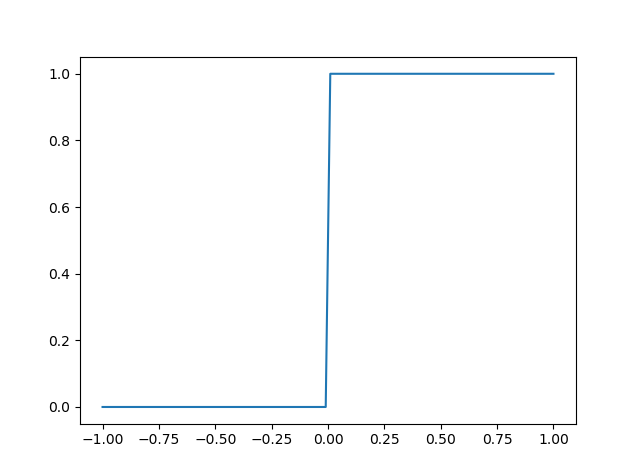
\includegraphics[scale=0.5]{assets/heaviside}
  \caption{La fonction échelon unité, ou fonction de Heaviside.}
  \label{fig:heaviside}
\end{figure}

Le but du perceptron est de modéliser le comportement du neurone biologique. 
Ce dernier est stimulé par des signaux qui lui parviennent par ses dendrites et, si 
la stimulation est suffisament importante, renvoie un signal à d'autres neurones au travers de son axone.

En notant $x_1, x_2, \dots, x_n$ ces stimulations, qui sont donc les entrées du perceptron, et 
$w_1, w_2, \dots, w_n$ les pondérations associées à ces entrées, on peut simplement exprimer le 
comportement du perceptron par :

\[
\text{sortie } =
\begin{cases}
 1 \text{ si } w \cdot x  \geq \text{ seuil} \\
 0 \text{ si } w \cdot x  < \text{ seuil.} 
 \end{cases}
\]

Par la suite, on préférera, plutôt que de considérer un seuil, considérer 
une quantité $b$ que l'on appelera biais définie par $b = -\text{seuil}$, et on écrira:

\[
\text{sortie } = H(w \cdot x + b)
\]

Les perceptrons peuvent être utilisés pour coder des fonctions logiques. 
Par exemple, en prenant $w = (1, 1)$ et $b = -2$, notre perceptron code 
un ET logique (avec la convention 0 pour FAUX et 1 pour VRAI).

\begin{figure}[h]
  \centering
  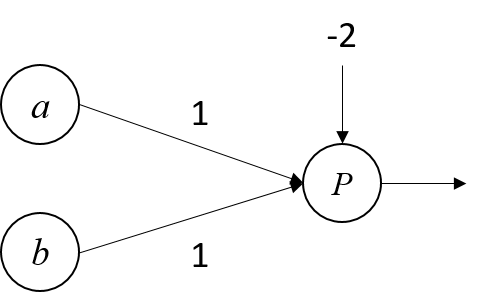
\includegraphics[scale=0.5]{assets/and-perceptron}
  \caption{Fonction ET logique.}
  \label{fig:and-perceptron}
\end{figure}

De même, en prenant $w = (-2, -2)$ et $b = 3$, on code la fonction NAND 
(négation du ET logique). Pour s'en convaincre, on peut dresser le tableau 
des sorties en fonctions de toutes les entrées possibles comme cela est fait 
dans la table \ref{table:nand-perceptron}.

\begin{table}[h]
  \centering
\begin{tabular}{|c|c|c|c|}
\hline
$x_1$ & $x_2$ & $wx + b$ & Sortie \\
\hline
0     & 0     & 3        & 1 \\  
0     & 1     & 1        & 1 \\  
1     & 0     & 1        & 1 \\  
0     & 0     & -1       & 0 \\   
\hline
\end{tabular} 
  \caption{Table de vérité du perceptron.}
  \label{table:nand-perceptron}
\end{table}

\begin{figure}[h]
  \centering
  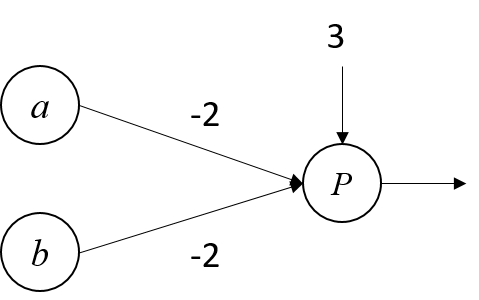
\includegraphics[scale=0.5]{assets/nand-perceptron}
  \caption{Fonction NAND.}
  \label{fig:nand-perceptron}
\end{figure}

Comme la fonction NAND permet de coder n'importe quelle fonction logique, 
on en déduit qu'en utilisant la sortie de perceptrons comme entrées d'autres 
perceptrons, on peut construire n'importe quelle fonction logique.

Exercice : Coder la fonction OU logique pour $n$ entrées.

Cette idée d'empiler des couches de perceptrons pour coder une fonction logique 
conduit naturellement à l'idée que l'on pourrait se faire d'un réseau de neurones.

\begin{figure}[h]
  \centering
  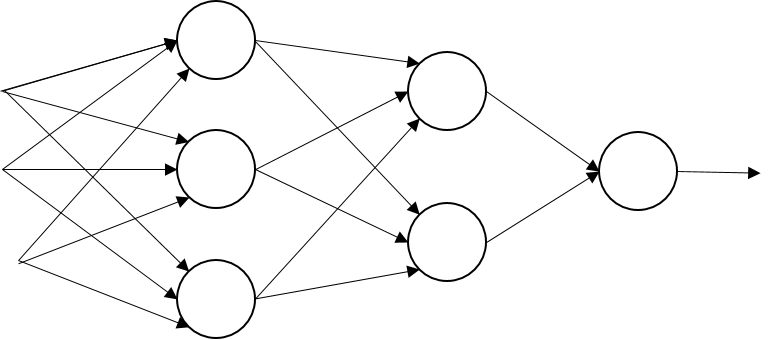
\includegraphics[scale=0.5]{assets/perceptron-network}
  \caption{Un réseau de perceptrons.}
  \label{fig:perceptron-network}
\end{figure}

Jusqu'à présent, nous nous sommes restreint à des entrées binaires (0 ou 1) 
codant des valeurs logiques. Ceci n'est pas nécessaire : les entrées d'un perceptron 
peuvent très bien être des réels.
Plaçons nous, pour les exemples qui vont suivres, dans $\mathbb{R}^2$. 
Pour chaque point $(x, y)$ du plan, on donnera $x$ comme première entrée d'un 
perceptron et $y$ comme seconde entrée. 
Le perceptron ayant pour paramètre $w=(\alpha_x, \alpha_y)$ et $b$ va alors 
séparer l'espace en deux plans par la droite d'équation $\alpha_y y + \alpha_x x + b = 0$. 
Les points tels que $\alpha_y y + \alpha_x x + b \geq 0$ auront pour sortie $1$, et 
les autres auront pour sortie $0$.

Ceci est illustré par la figure \ref{fig:perceptron-example1} dans laquelle la 
partie verte correspond à une sortie positive du perceptron dès lors que $y \geq x$.

\begin{figure}[h]
  \centering
  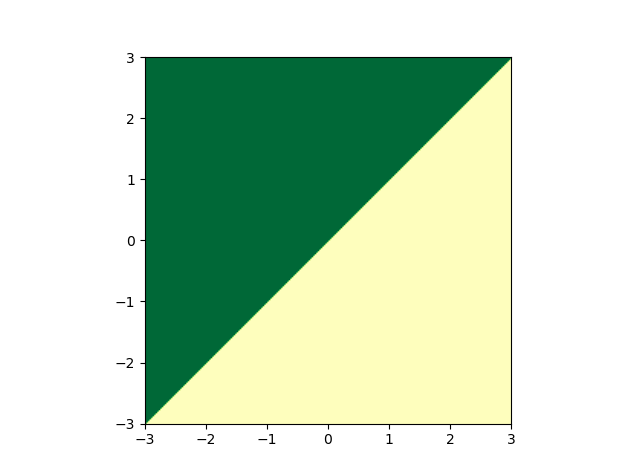
\includegraphics[scale=0.5]{assets/perceptron-example1}
  \caption{Découpage du plan en deux par un perceptron.}
  \label{fig:perceptron-example1}
\end{figure}


En utilisant plusieurs perceptron, on va pouvoir effectuer plusieurs sous-découpage 
de l'espace, et en utilisant un ET logique dans une dernière couche 
on va pouvoir récuperer la partie de l'espace 
correspondant à l'intersection de toutes les parties correspondants aux sorties 
positives des perceptrons de la couche précédente.

\begin{figure}[h]
  \centering
  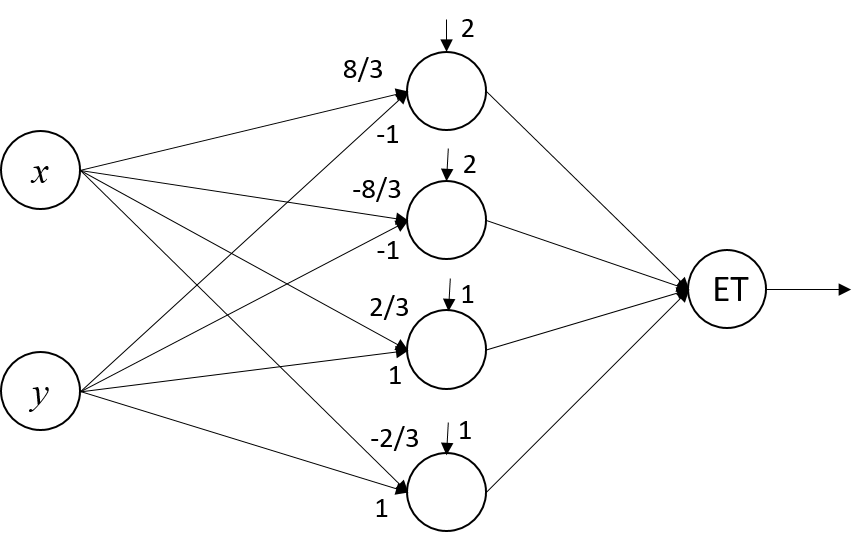
\includegraphics[scale=0.5]{assets/perceptron-network-example2}
  \caption{Un premier réseau de perceptrons.}
  \label{fig:perceptron-network-example2}
\end{figure}

\begin{figure}[h]
  \centering
  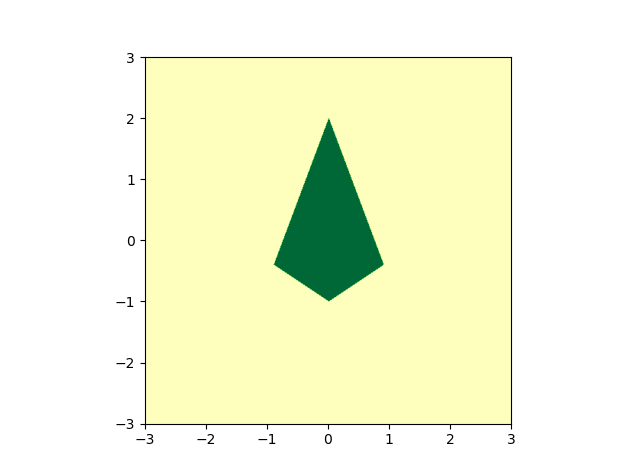
\includegraphics[scale=0.5]{assets/perceptron-example2}
  \caption{Découpage du plan par un réseau de perceptrons.}
  \label{fig:perceptron-example2}
\end{figure}

Cette approche a ses limites car elle ne permet d'obtenir qu'une partie convexe 
du plan. Pour obtenir des parties plus complexes (e.g.\/ non convexes, ou non 
fortement connexes), on peut utiliser d'autres fonctions logiques, comme le OU. 

\begin{figure}[h]
  \centering
  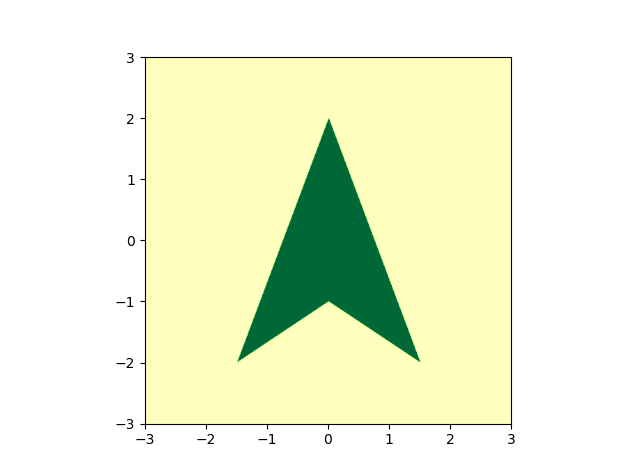
\includegraphics[scale=0.5]{assets/perceptron-example3}
  \caption{Un découpage non convexe du plan avec un réseau de perceptrons à deux couches.}
  \label{fig:perceptron-example3}
\end{figure}

Il n'est pas difficile d'imaginer que l'on puisse étendre ce que l'on vient de faire en 
2 dimensions à un nombre plus grand de dimensions; et avec un non plus une seule sortie 
mais plusieurs (correspondant par exemple chacune à une classe, à un chiffre que l'on 
souhaite reonnaître).
On pourrait donc en théorie construire un réseau de neurones avec des perceptrons 
qui serait capable de reconnaître des chiffres. 
L'un des problèmes de cette approche est qu'il faudrait déjà connaître les coefficients 
(ou paramètres) de l'ensemble des perceptrons du réseau.
On pourrait alors avoir envie d'écrire un algorithme permettant de construire un tel 
réseau. On peut imaginer plusieurs principes pour cet algorithme :`
\begin{enumerate}
  \item tester tous les coefficients possibles pour les perceptrons;
  \item partir d'une configuration aléatoire et modifier petit à petit les coefficients 
        jusqu'à obtenir un résultat satisfaisant.
\end{enumerate}

La première idée est tout simplement irréalisable car il y a une infinité de valeurs 
possibles pour chaque coefficient du réseau. On pourrait penser à prendre une 
approche probabiliste en testant un certains nombres de réseau et en espérant tomber sur 
un bon; ce qui paraît néanmoins très improbable ! 
La deuxième idée n'est également pas envisageable car elle souffre d'un problème difficile 
à gérer. La discontinuité de la fonction de Heaviside fait qu'un petit changement de coefficient 
peut faire passer la sortie d'un neurone de 0 à 1 ce qui peut correspondre à un changement 
significatif de l'entrée des neurones de la couche suivante. Il est donc compliqué d'évaluer 
l'impact d'un changement à une couche donnée sur les couches qui suivent.

L'idée qui va être exploré dans les paragraphes suivants est d'utiliser une autre fonction, 
appelée fonction d'activation, que la fonction échelon d'Heaviside; et de faire en sorte que 
cette fonction d'activation soit dérivable (et donc continue) pour pouvoir utiliser des 
résultats d'analyse et pouvoir ainsi estimer l'impact du changement d'un coefficient.
On sera alors en mesure de modifier un réseau généré aléatoirement pour le faire résoudre 
notre problème de classification (on parlera d'apprentissage).



\section{Structure des réseaux de neurones}



\begin{definition}[Fonction sigmoïde]
On appelle fonction sigmoïde la fonction définie de $\mathbb{R}$ dans $[0, 1]$ par :
\[
\sigma(x) = \frac{1}{1 + e^{-x}}
\]
\end{definition}

On notera que $\lim_{x \to +\infty} \sigma(x) = 1$ et $\lim_{x \to -\infty} \sigma(x) = 0$. 
Ainsi, asymptotiquement, la fonction sigmoïde à le même comportement que la fonction 
de Heaviside.

Entre les deux, on à un comportement qui diffère fortement du perceptron avec notamment 
la non discontinuité en 0 et $\sigma(0) = \frac{1}{2}$. 
Dans le cadre de notre utilisation pour la classification on aura tendance 
à considérer que la sortie du neurone est à \textsc{vrai} dès qu'elle sera supérieure 
à une certaine valeur (typiquement $\frac{1}{2}$).

On a également quelques propriétés intéressantes de symétrie. En effet,

\[
\sigma'(x) = \frac{e^{-x}}{1 + e^{-x}} = \sigma(x) (1 - \sigma(x))
\]

\[
\sigma'(x) - \sigma'(-x) = \frac{e^{-x}(e^{2x} + 2 e^{x} + 1) - e^{x}(e^{-2x} + 2 e^{-x} + 1)}{(1+e^{-x})^2 (1+e^{x})^2} = 0
\]

ce qui signifie que la sigmoïde admet pour centre de symétrie le point $(0, \frac{1}{2})$.

Cette fonction a de plus l'avantage d'être dérivable en tout point (et de dérivée non nulle), 
ce qui nous servira plus tard dans le cadre de l'apprentissage.


\begin{definition}[Modélisation d'un neurone]
En notant $b$ le biais du neurone, $w$ son vecteur des poids et $\sigma$ sa fonction 
d'activation, on peut écrire la sortie $y$ d'un neurone en fonction de son entrée $x$ 
de la manière suivante:
\[
y = \sigma(w \cdot x + b)
\]
\end{definition}


\begin{definition}[Vectorisation d'une fonction]
Soit $f$ une fonction de $\mathbb{R} \mapsto \mathbb{R}$. 
On pose pour tout vecteur $x$ de $\mathbb{R}^n$ :
\[
f(x) = 
\begin{pmatrix}
f(x_1) \\
f(x_2) \\
\vdots \\
f(x_n)
\end{pmatrix}
\]
On dit que l'on vectorise la fonction $f$.
\end{definition}

\textbf{Achtung !} Par abus de notation, on utilise encore le nom de $f$ pour désigner 
cette fonction, mais il s'agit bien d'une fonction différente puisqu'elle est à valeurs 
de $\mathbb{R}^n$ dans $\mathbb{R}^n$. Cet abus nous est néanmoins utile pour définir 
simplement les couches d'un réseau de neurones.

On considère dans les définitions suivantes une couche d'un réseau de neurones 
constituée de $n$ neurones. On note $w_i$ le vecteur des poids associé à chaque neurone.
On a alors la définition suivante:
 
\begin{definition}[Matrice des poids]
En notant $w_i$ les vecteurs des poids de $n$ neurones, on définit par blocs 
la matrice $w$ des poids:
\[
w = 
\begin{pmatrix}
{w_1}^T \\
{w_2}^T \\
\vdots \\
{w_n}^T
\end{pmatrix}
\]
\end{definition}

On définit de manière analogue un vecteur des biais.

\begin{definition}[Vecteur des biais]
En notant $b_i$ les biais de $n$ neurones, on définit le vecteur des biais 
d'une couche d'un réseau de neurones par:
\[
b = 
\begin{pmatrix}
{b_1} \\
{b_2} \\
\vdots \\
{b_n}
\end{pmatrix}
\]
\end{definition}

On a alors la proposition suivante:

\begin{proposition}[Ecriture matricielle d'une couche]
Soit une couche d'un réseau constituée de $n$ neurones et ayant pour matrice 
des poids $w$ et pour vecteur des biais $b$. Si les neurones ont tous la même 
fonction d'activation $\sigma$, on peut écrire les sorties des neurones sous la 
forme d'un vecteur $y$ vérifiant:
\[
y = \sigma(w \cdot x + b)
\]
où les $y_i$ correspondent à la sortie du neurones $i$.
\end{proposition}

On notera que dans cette proposition, on utilise la version vectorisée de $\sigma$.
Une écriture équivalente est:
\[
\begin{pmatrix}
  y_1 \\
  y_2 \\
  \vdots \\
  y_n
\end{pmatrix}
 = 
\begin{pmatrix}
  \sigma(w_1 \cdot x + b_1) \\
  \sigma(w_2 \cdot x + b_2) \\
  \vdots \\
  \sigma(w_n \cdot x + b_n)
\end{pmatrix}
\]

En fait, cette écriture est identique à celle d'un unique neurone !
Elle est également intéressante d'un point de vue computationnelle : au lieu 
de calculer une à une les sorties des neurones, il est plus efficace de faire 
un calcul matriciel (les bibliothèques étant en générales optimisées pour cela).
Cela permet également d'avoir un code plus simple (avec notamment moins de boucles).

\section{Apprentissage par la descente de gradient}



\section{L'algorithme de rétro-propagation}


